%%%%%%%%%%%%%%%%%%%%%%%%%%%%%%%%%%%%%%%%%%%%%%%%%%%%
% This will help you in writing your homebook
% Remember that the character % is a comment in latex
%
% chapter 6
\chapter{Synthesis and Place \& Route}
\label{cha6}

\section{Shynthesis}

The two different designs have been synthesized using Synopsys Design Compiler, in order to obtain the maximum working frequency and an area estimation of the circuits.
The following \hyperref[tab:performance]{table} summarizes the obtained results.  
\\
\begin{table}[h!]
    \centering
    \begin{tabular}{m{3cm} m{3cm} m{3cm}}
    \hline
         & \textbf{RISCV} & \textbf{Modified RISCV}\\
         \hline
         \textbf{Min. Period} & 3.55 ns & 3.6 ns\\
         \textbf{Max. Frequency} & 281.7 MHz& 277.8 MHz \\
         \textbf{Area} & 14006.23 $\mu$m$^{2}$ & 14802.1 $\mu$m$^{2}$ \\
         \hline
    \end{tabular}
    \caption{\textbf{Design Compiler Reports}}
    \label{tab:performance}
\end{table}

As expected, the modified design with the added component occupies more area. Moreover, since the added hardware is placed along the critical path, 
the maximum frequency is also slightly lower; however this is compensated by the reduced time needed for the computation of the instruction.

The report of the \emph{elaborate} command lists the inferred memory devices inserted in the netlist. Every element was checked to avoid the insertion of latch instead of 
flip-flops.
Finally, both synthesized netlists were simulated with Modelsim to confirm they still behaved correctly.

\section{Place \& Route}

After the synthesis of the circuits, place \& route was performed using Cadence Innovus. This requires to perform the following steps:

\begin{itemize}
    \item Importing the design;
    \item Floorplanning;
    \item Power planning and routing;
    \item Cell placing;
    \item Signal routing;
    \item Timing and design analysis.
\end{itemize}

The procedure returned no violations in connections and geometry. The resulting netlist was saved together with the final gate count.

\begin{table}[h!]
    \centering
    \begin{tabular}{m{3cm} m{3cm} m{3cm}}
    \hline
         & \textbf{RISCV} & \textbf{Modified RISCV}\\
         \hline
         \textbf{Area} & 13533.0 $\mu$m$^{2}$ & 14133.6 $\mu$m$^{2}$ \\
         \hline
    \end{tabular}
    \caption{\textbf{Innovus Reports}}
    \label{tab:performance}
\end{table}

Innovus was able to optimize the netlists and save a noticeable amount of area on both designs, with respect to the value obtained with Synopsys.
Also in this case, the produced netlists were simulated to verify the compliance with the original design.

\begin{figure}[!h]
    \centering
    \begin{subfigure}[b]{0.45\linewidth}
      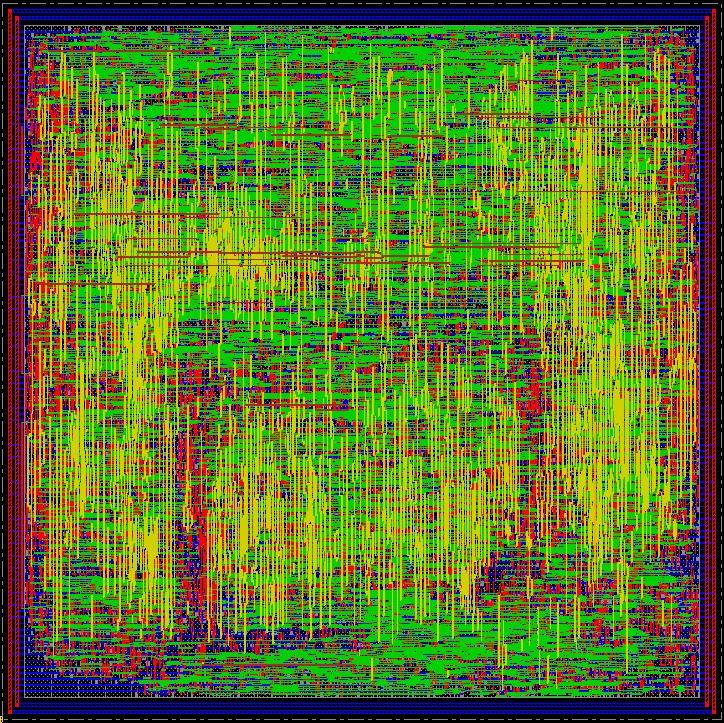
\includegraphics[width=\linewidth]{chapters/chap6images/riscv.jpg}
      \caption{RISCV}
    \end{subfigure}
    \begin{subfigure}[b]{0.452\linewidth}
      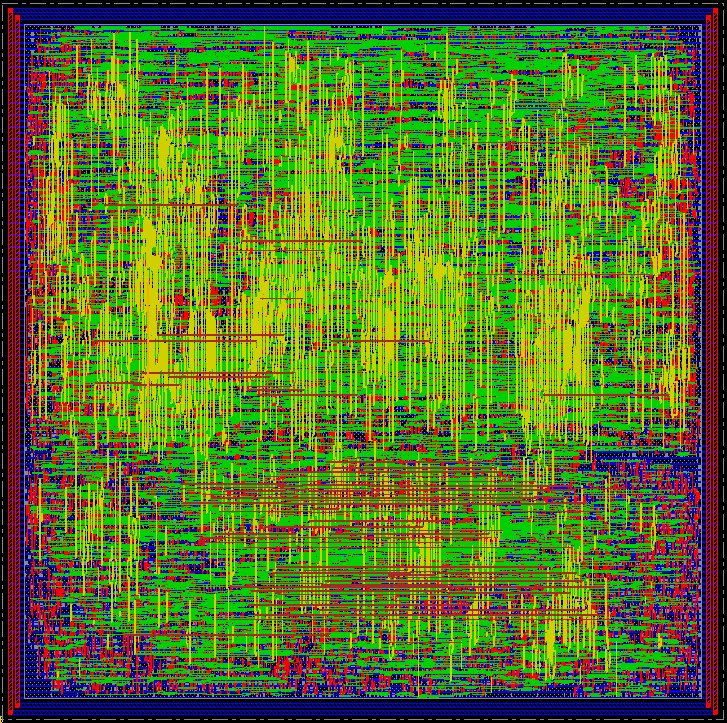
\includegraphics[width=\linewidth]{chapters/chap6images/riscv_abs.jpg}
      \caption{Modified RISCV}
    \end{subfigure}
    \caption{\textbf{Place and route of the two designs}}
    \label{fig:placeroute}
\end{figure}